\documentclass[handout,compress]{beamer}

\usetheme[block=fill]{metropolis}

\usepackage{graphicx} % Allows including images
\usepackage{amsmath,amsfonts,amsthm,amssymb}
\usepackage{color}
\usepackage{xcolor,cancel}
%\setitemize{label=\usebeamerfont*{itemize item}%
%	\usebeamercolor[fg]{itemize item}
%	\usebeamertemplate{itemize item}}
\definecolor{mDarkBrown}{HTML}{604c38}
\definecolor{mDarkTeal}{HTML}{23373b}
\definecolor{mLightBrown}{HTML}{EB811B}
\definecolor{mMediumBrown}{HTML}{C87A2F}
\definecolor{mygreen}{HTML}{98C2B9}
\definecolor{myyellow}{HTML}{DFD79C}
\definecolor{myblue}{HTML}{8CA7CC}
\definecolor{kern}{HTML}{8CC2B7}

\usepackage{float}
\usepackage{framed}
\usepackage{epsfig}
\usepackage{graphicx}
\usepackage{subcaption}
\usepackage{ulem}
\usepackage{hhline}
\usepackage{multirow}
\usepackage{comment}   
\usepackage{bbm}
\usepackage{tikz}   
\usepackage{ulem}
\def\Put(#1,#2)#3{\leavevmode\makebox(0,0){\put(#1,#2){#3}}}
\newcommand*\mystrut[1]{\vrule width0pt height0pt depth#1\relax}
\newcommand{\eqdef}{\mathbin{\stackrel{\rm def}{=}}}


\newcommand{\bs}[1]{\boldsymbol{#1}}
\newcommand{\bv}[1]{\mathbf{#1}}
\newcommand{\R}{\mathbb{R}}
\newcommand{\E}{\mathbb{E}}

\DeclareMathOperator*{\argmin}{arg\,min}
\DeclareMathOperator*{\argmax}{arg\,max}
\DeclareMathOperator{\nnz}{nnz}
\DeclareMathOperator{\Var}{Var}
\DeclareMathOperator{\sinc}{sinc}
\DeclareMathOperator{\mv}{mv}
\DeclareMathOperator{\sgn}{sgn}
\DeclareMathOperator{\step}{step}
\DeclareMathOperator{\gap}{gap}
\DeclareMathOperator{\poly}{poly}
\DeclareMathOperator{\tr}{tr}
\DeclareMathOperator{\orth}{orth}
\newcommand{\norm}[1]{\|#1\|}
\captionsetup[subfigure]{labelformat=empty}
\captionsetup[figure]{labelformat=empty}
\DeclareMathOperator*{\lmin}{\lambda_{min}}
\DeclareMathOperator*{\lmax}{\lambda_{max}}

\newcommand{\specialcell}[2][c]{%
  \begin{tabular}[#1]{@{}c@{}}#2\end{tabular}}
\newcommand{\specialcellleft}[2][c]{%
\begin{tabular}[#1]{@{}l@{}}#2\end{tabular}
}

\usepackage{tabstackengine}
\stackMath

\newtheorem{claim}[theorem]{Claim}


%----------------------------------------------------------------------------------------
%	TITLE PAGE
%----------------------------------------------------------------------------------------

\title{CS-UY 4563: Lecture 12 \\ k-Nearest Neighbors, Kernel Methods}
\author{NYU Tandon School of Engineering, Prof. Christopher Musco}
\date{}

\begin{document}

\begin{frame}
	\titlepage 
\end{frame}

\metroset{titleformat=smallcaps}

\begin{frame}
	\frametitle{course admin}
	\begin{itemize}
		\item Lab 4 due on \textbf{Friday, at 11:59pm}. Requires correct solution to HW3, Problem 2. I will post this after class. 
		\item Short lab on Gradient Descent will be released soon and due after break. 
		\item Upcoming labs involve image data and require more programming. Made up with lighter written homework.
	\end{itemize}
\end{frame}

\begin{frame}
	\frametitle{course project}
	Break is a great time to start mulling over ideas for your course project!
	Details in \texttt{project\_guidelines.pdf}.
	\begin{enumerate}
		\item Find or collect a data set.
		\item Ask a question (or two) about the data set which can possibly be answered with machine learning. 
		\item Apply tools and techniques learned in the class to answering that question. 
	\end{enumerate}
\end{frame}

\begin{frame}
	\frametitle{course project}
	\begin{itemize}
		\item Must work in \textbf{groups of 2}. Coordinate over Piazza if looking for a partner. 
		\item Any data set or topic is allowed, but youo should not reproduce an analysis that has already been done! Ask a new question or take a new approach. 
		\item Talk to me or the TA's \emph{early} if you are stuck on coming up with an idea, or need help narrowing down options. 
	\end{itemize}
\end{frame}

\begin{frame}
		\frametitle{course project}
			\textbf{4/1, Choose Project Partner and Topic.} Email me.
			
			\textbf{4/2,4/6-4/8, Schedule Mandatory Meeting.} Claim a time-slot in the Google Doc linked in the project information document. 
			
			\textbf{4/13, Project Proposal Due.} 2 Pages. Need to have dataset finalized! 
			
			\textbf{5/6, 5/11, Project Presentations in Class.} 5 Minutes. 
			
			\textbf{5/11, Final Report Due} 4+ Pages. 
\end{frame}

\begin{frame}
		\frametitle{project tips}
		\textbf{Look at your data!} Plot features, examine full examples, look for missing data or inconsistencies. 
		
		\textbf{Start small.} Test and debug code on a \emph{small subset} of your data before running on the whole thing. 
		
		\textbf{Start simple.} Try the simplest methods first. Linear regression, naive Bayes, etc. Even simpler: for regression, predict using $\text{mean}(\vec{y})$. For classification predict using $\max{\vec{y}}$ (the most common label). \textbf{You need to develop a baseline to compare your methods against.}
\end{frame}

\begin{frame}
	\frametitle{$k$-nearest neighbor method}
	\textbf{$k$-NN algorithm:} a simple but powerful baseline for classification.
	
	\textbf{Training data:} $(\vec{x}_1, y_1), \ldots, (\vec{x}_n, y_n)$ where $y_1, \ldots, y_n \in \{1,\ldots, q\}$. 
	
	\textbf{Classification algorithm:}
	
	Given new input $\vec{x}_{new}$,
	\begin{itemize}
		\item Compute $sim(\vec{x}_{new}, \vec{x}_1), \ldots, sim(\vec{x}_{new}, \vec{x}_n).$\footnote{$sim(\vec{x}_{new}, \vec{x}_i)$ is any chosen \emph{similarity function}, like $1 - \|\vec{x}_{new} - \vec{x}_i\|_2$.}
		\item Let $\vec{x}_{j_1}, \ldots, \vec{x}_{j_k}$ be the training data vectors with highest similarity to $\vec{x}_{new}$. 
		\item Predict $y_{new}$ as $majority(y_{j_1}, \ldots, y_{j_k})$.
	\end{itemize}
\end{frame}

\begin{frame}
	\frametitle{$k$-nearest neighbor method}
	\begin{center}
		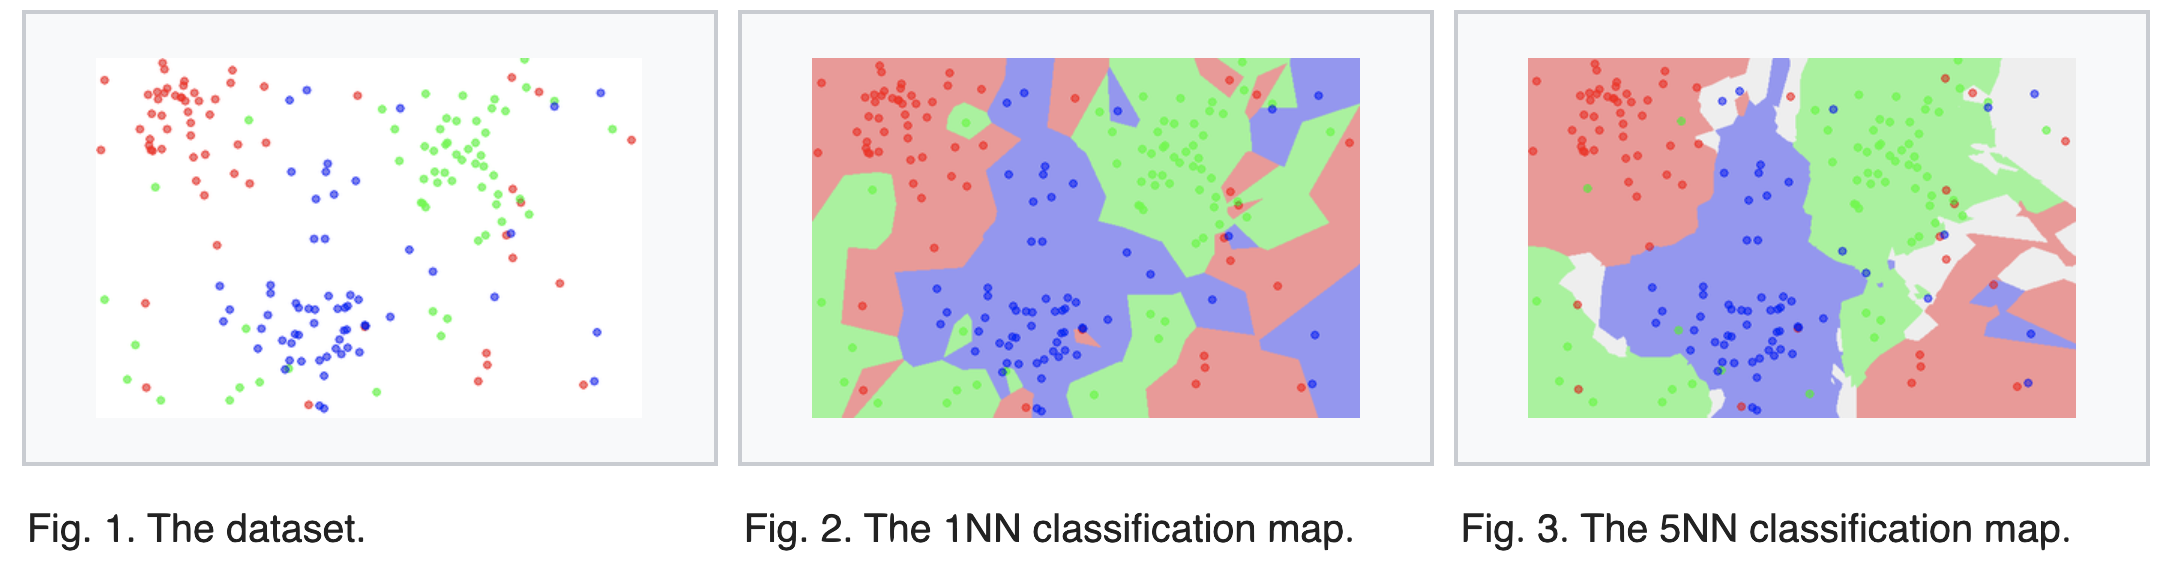
\includegraphics[width=\textwidth]{knn.png}
	\end{center}
	\begin{itemize}
		\item Smaller $k$, more complex classification function.
		\item Larger $k$, more robust to noisy labels. 
	\end{itemize}
\begin{center}
	\textbf{Works remarkably well for many datasets.}
\end{center}
\end{frame}

\begin{frame}
	\frametitle{mnist image data}
	Especially good for large datasets with lots of repetition. Works well on MNIST for example:
	\begin{center}
		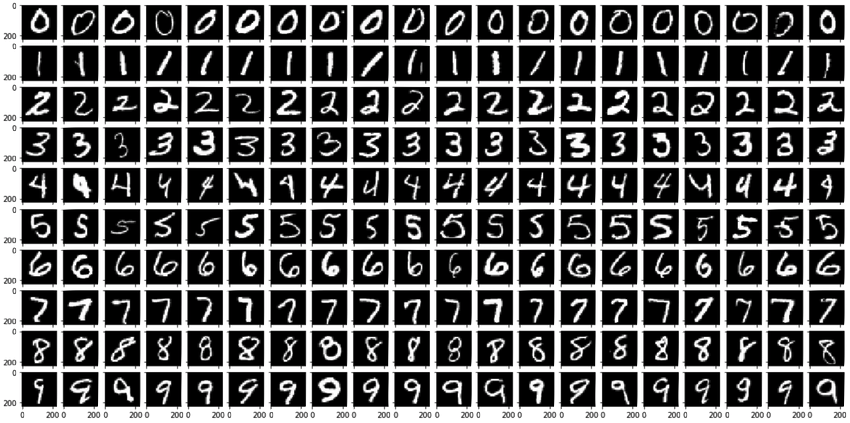
\includegraphics[width=.6\textwidth]{mnist.png}
		
		\textbf{\alert{$\approx 95\%$ Accuracy out-of-the-box.}}\footnote{Can be improved to $99.5\%$ with some simple tricks!}
	\end{center}


	Let's look into this example a bit more...
	\vspace{3em}
\end{frame}

\begin{frame}
	\frametitle{mnist image data}
	Each pixel is number from $[0,1]$. $0$ is black, $1$ is white. 
	Represent $28\times 28$ matrix of pixel values as a flattened vector.
	\begin{center}
		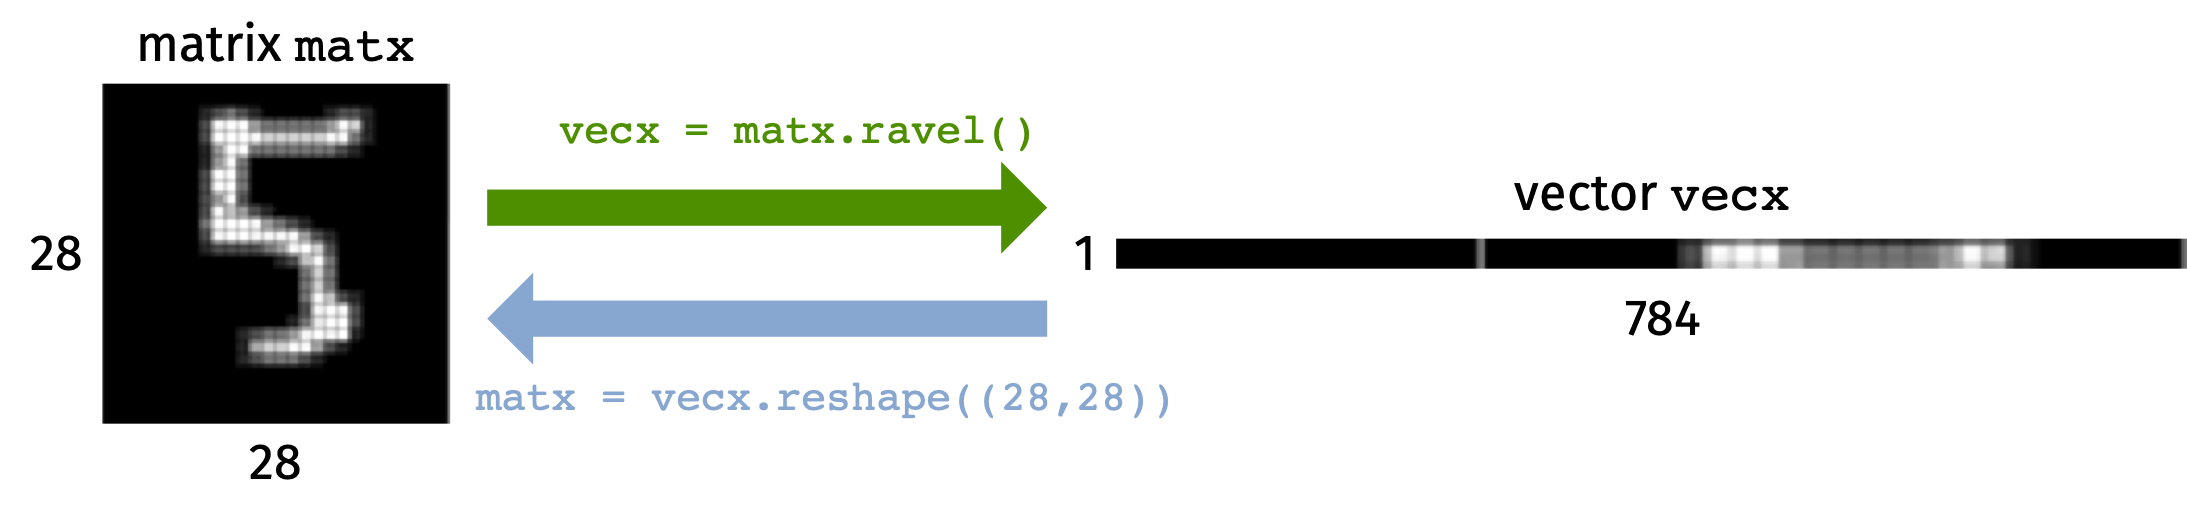
\includegraphics[width=\textwidth]{flatten.png}
		
		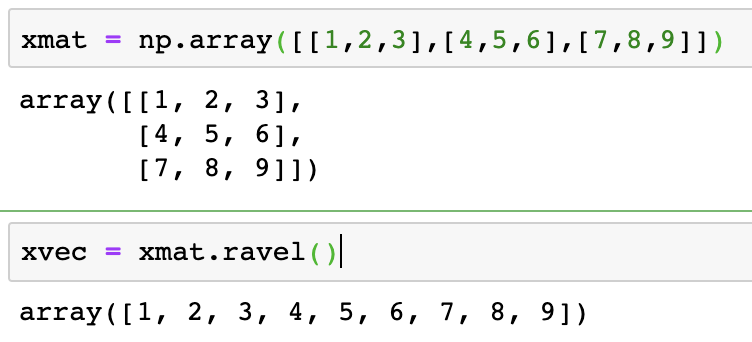
\includegraphics[width=.7\textwidth]{flatten_code.png}
	\end{center}
\end{frame}

\begin{frame}
	\frametitle{inner product similarity}
	Given data vectors $\vec{x},\vec{w}\in \R^d$, the inner product $\langle\vec{x}, \vec{w}\rangle$ is a natural similarity measure.
	\begin{align*}
	\langle\vec{x}, \vec{w}\rangle = \sum_{i=1}^d \vec{x}[i]\vec{w}[i] = \cos(\theta)\|\vec{x}\|_2\|\vec{w}\|_2.
	\end{align*}
		\begin{center}
		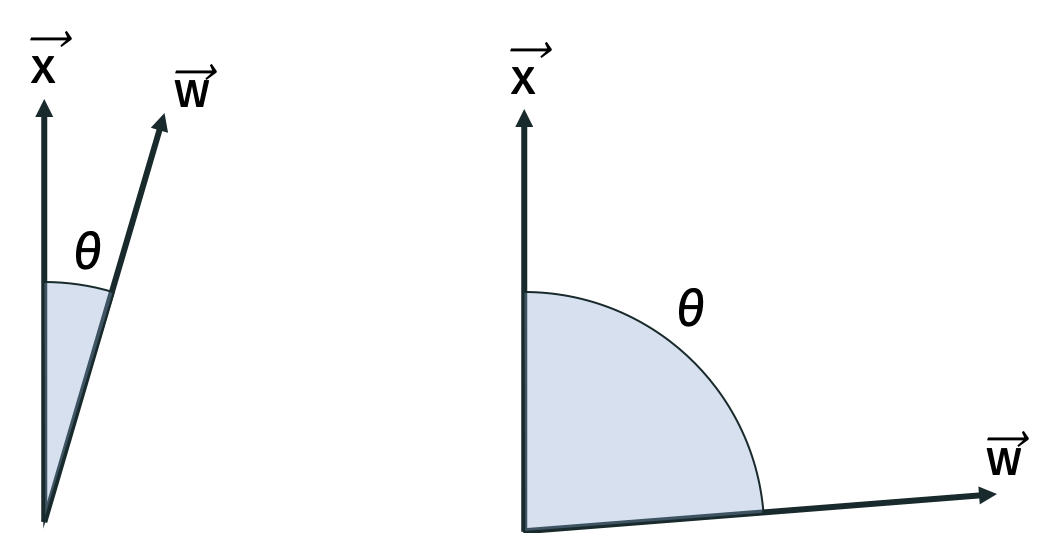
\includegraphics[width=.7\textwidth]{inner_product_similarity.png}
	\end{center}
\end{frame}

\begin{frame}
	\frametitle{inner product similarity}
	Connection to Euclidean ($\ell_2$) Distance:
	\begin{align*}
	\|\vec{x} - \vec{w}\|_2^2 = \|\vec{x}\|_2^2 + \|\vec{w}\|_2^2 \alert{- 2\langle\vec{x}, \vec{w}\rangle}
	\end{align*}
	For a set of vectors with the same norm, the pair of vectors with \emph{largest inner product} is the pair with \emph{smallest Euclidean distance}. 
\end{frame}

\begin{frame}
	\frametitle{inner product for mnist}
	Inner product between MNIST digits:
	\begin{center}
			
\includegraphics[width=.8\textwidth]{flat_compare.png}
	\begin{align*}
	\langle \vec{x},\vec{w}\rangle = \sum_{i=1}^{28} \sum_{j=1}^{28} \texttt{matx}[i,j]\texttt{matw}[i,j].
	\end{align*}
	\end{center}
	Inner product similarity is higher when the images have large pixel values (close to $1$) in the same locations. I.e. when they have a lot of overlapping white/light gray pixels.
\end{frame}

\begin{frame}
	\frametitle{inner product for mnist}
	\textbf{Visualizing the inner product between two images:}
		\begin{center}
			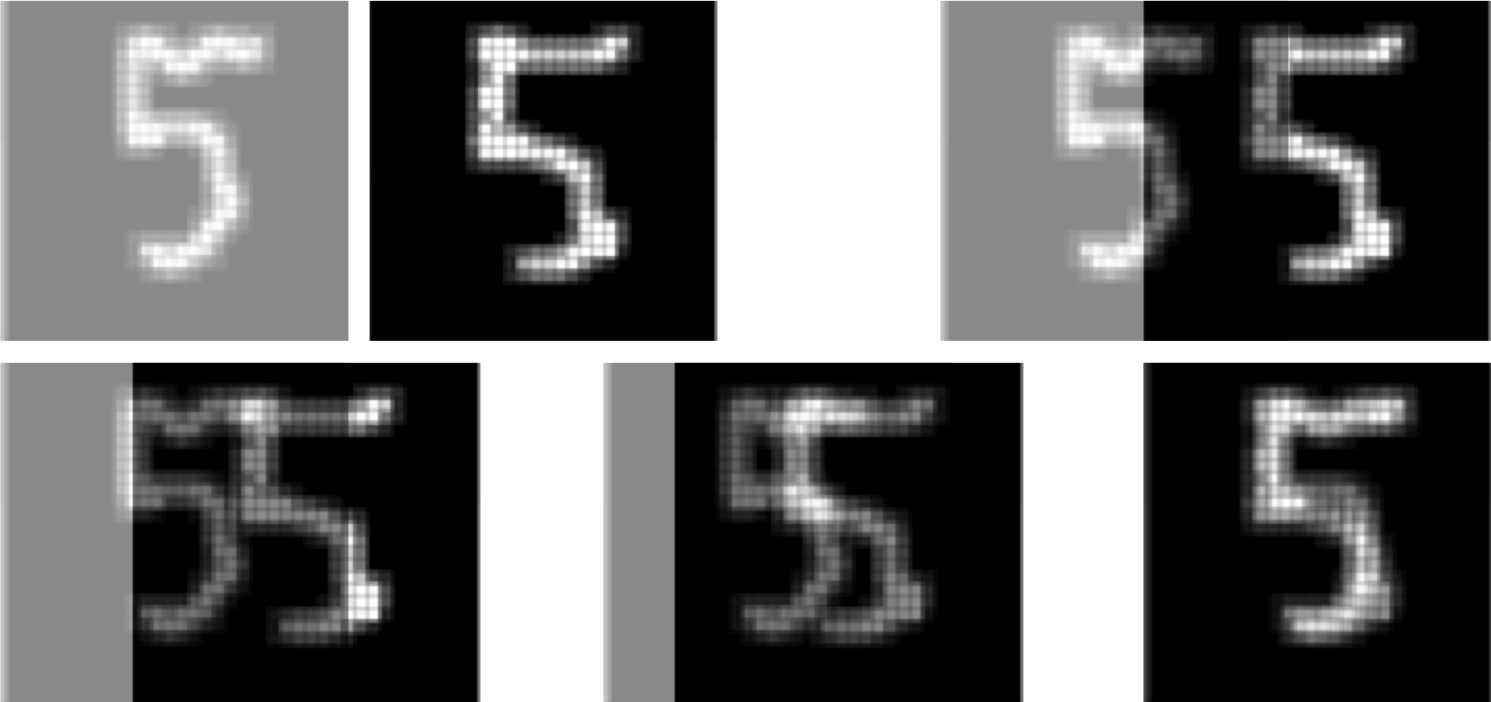
\includegraphics[width=.8\textwidth]{innerproduct_visualizatoin.png}
		\end{center}
	Images with high inner product have a lot of overlap.
\end{frame}

\begin{frame}
	\frametitle{k-nn algorithm on mnist}
	\textbf{Most similar images during $k$-nn search, $k=9$:}
	\begin{center}
		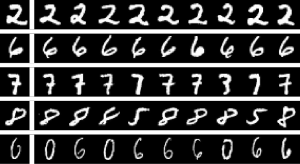
\includegraphics[width=.5\textwidth]{MNISTknn.png}
	\end{center}
\end{frame}

\begin{frame}
	\frametitle{k-nn for other images}
	Does not work as well for less standardized classes of images:
	\begin{center}
		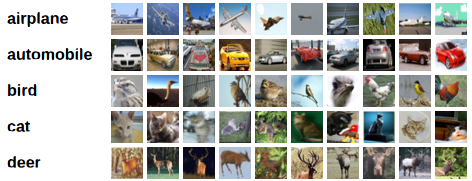
\includegraphics[width=.8\textwidth]{cifar10.png}
		
		CIFAR 10 Images
	\end{center}
	Even after scaling to have same size, converting to separate RGB channels, etc. something as simple as $k$-nn won't work.
\end{frame}

\begin{frame}
	\frametitle{another view on logistic regression}
	\textbf{One-vs.-all Classification with Logistic Regression:}
	\begin{itemize}
		\item Learn $q$ classifiers with parameters $\vec{\beta}_1, \vec{\beta}_2, \ldots, \vec{\beta}_q$.
		\item Given $\vec{x}_{new}$ compute $\langle \vec{x}_{new}, \vec{\beta}_1\rangle, \ldots, \langle\vec{x}_{new}, \vec{\beta}_q\rangle$
		\item Predict class $y_{new} = \argmax_i \langle\vec{x}_{new}, \vec{\beta}_i\rangle$.
	\end{itemize}
	If each $\vec{x}$ is a vector with $28\times 28 = 784$ entries than each $\vec{\beta}_i$ also has $784$ entries. Each parameter vector can be viewed as a $28\times 28$ image. 
\end{frame}

\begin{frame}
	\frametitle{matched filter}
	Visualizing $\vec{\beta}_1, \ldots, \vec{\beta}_q$:
	\begin{center}
		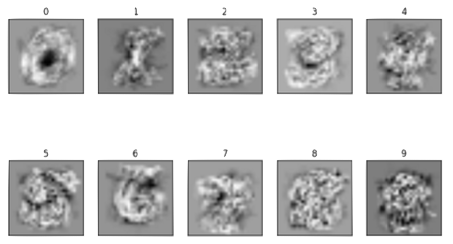
\includegraphics[width=.7\textwidth]{logweights.png}
	\end{center}
For an input image \hspace{.5em}
\includegraphics[width=.05\textwidth]{five.png}\hspace{.5em}, compute \emph{inner product} similarity with all weight matrices and choose most similar one. 

In contrast to $k$-NN, only need to compute similarity with $q$ items instead of $n$.
\end{frame}

\begin{frame} 
	\frametitle{alternative view}
	\textbf{Logistic Regression Model:}
	
	Given data matrix $\bv{X} \in \R^{n\times d}$ (here $d = 784$) and binary label vector $\vec{y}\in \{0,1\}^n$ for class $i$ (1 if in class $i$, 0 if not), find $\vec{\beta} \in \R^d$ to minimize the log loss between:
	\begin{align*}
	&\vec{y} & &\text{and} & h(\bv{X}\vec{\beta})
	\end{align*}
	where $h(z) = \frac{1}{1 + e^{-z}}$ applies the logistic function entrywise to $\bv{X}\vec{\beta}$. 
	
	
	Loss = $-\sum_{j=1}^n y_j\log(h(\bv{X}\vec{\beta})_j) +  (1-y_j)\log(1- h(\bv{X}\vec{\beta})_j)$
	
\end{frame}

\begin{frame} 
	\frametitle{alternative view}
		\textbf{Logistic Regression Model:}
	
	Given data matrix $\bv{X} \in \R^{n\times d}$ (here $d = 784$) and binary label vector $\vec{y}\in \{0,1\}^n$ for class $i$ (1 if in class $i$, 0 if not), find $\vec{\beta} \in \R^d$ to minimize the log loss between:
	\begin{align*}
	&\vec{y} & &\text{and} & h(\bv{X}\vec{\beta})
	\end{align*}
	
		
	\textbf{Reminder from linear algebra:}
	Without loss of generality, can assume that $\vec{\beta}$ lies in the \emph{row span} of $\bv{X}$. 
	
	So for any $\vec{\beta} \in \R^d$, there exists a vector $\vec{\alpha}\in \R^n$ such that:
	\begin{align*}
	\vec{\beta} = \bv{X}^T \vec{\alpha}.
	\end{align*}
	
\end{frame}

\begin{frame} 
	\frametitle{alternative view}
	\textbf{Logistic Regression Equivalent Formulation:}
	
	Given data matrix $\bv{X} \in \R^{n\times d}$ (here $d = 784$) and binary label vector $\vec{y}\in \{0,1\}^n$ for class $i$ (1 if in class $i$, 0 if not), \alert{\emph{find $\vec{\alpha} \in \R^n$}} to minimize the log loss between:
	\begin{align*}
	&\vec{y} & &\text{and} & h(\bv{X}\bv{X}^T\vec{\alpha}).
	\end{align*}
	
	Can still be minimized via gradient descent:
	\begin{align*}
		\nabla L(\vec{\alpha}) = \bv{X}\bv{X}^T(h(\bv{X}\bv{X}^T\vec{\alpha}) - \vec{y}).
	\end{align*}
	
\end{frame}

\begin{frame} 
	\frametitle{reformulated view}
	What does classification for a new point $\vec{x}_{new}$ look like?
	
	\begin{itemize}
	\item Learn $q$ classifiers with parameters $\vec{\alpha}_1, \vec{\alpha}_2, \ldots, \vec{\alpha}_q$.
	\item Given $\vec{x}_{new}$ compute $\langle \vec{x}_{new}, \bv{X}^T\vec{\alpha}_1\rangle, \ldots, \langle\vec{x}_{new}, \bv{X}^T\vec{\alpha}_q\rangle$
	\item Predict class $y_{new} = \argmax_i \langle\vec{x}_{new}, \bv{X}^T\vec{\alpha}_i\rangle$.
\end{itemize}
	
\end{frame}

\begin{frame} 
	\frametitle{reformulated view}
	\begin{align*}
	\langle\vec{x}_{new}, \bv{X}^T\vec{\alpha}\rangle = \sum_{j=1}^n \alpha_j \langle\vec{x}_{new}, \vec{x}_j\rangle.
	\end{align*}
	Similar to $k-NN$ classifier but we learn a \emph{weight} $\alpha_i$ for every $\vec{x}_i$ in our training set -- can be positive or negative. 
	
\end{frame}

\begin{frame} 
	\frametitle{kernel functions}
	
\end{frame}

\begin{frame} 
	\frametitle{kernel functions}
	
\end{frame}

\begin{frame} 
	\frametitle{kernel functions}
	
\end{frame}


\end{document} 






